\section{Center Based Per Axis Randomization}
\par Generating new points can be improved by randomizing based on a central point in the search space. Points far from the center point should be generated at lesser quantities and points near the center should be generated at greater quantities. \textbf{This section focuses on a new center based randomization method that improves finding more points that are either near or far a ``hotspot'' or a central point \cite{strategy}.} 

\par In the algorithm, nomads either stay in their positions doing nothing or reset to a new position in every iteration. This can be improved by introducing a new randomization method that can randomize a new position based on the previous position. In this improvement, Nomad lions either roam around a place to ``stay'' or find a new place.

\par The nomad lion roaming can be improved by changing the nomad lion roaming equation to
\begin{align*}
 \text{Lion'}_{ij} =
  \begin{cases}
   \text{RANDC}(\text{Lion}_{ij})        & \text{if rand}(0,1)  > pr_i \\
   \text{RAND}_j        & \text{otherwise}
 \end{cases}
\end{align*}
such that RANDC is a new function to be added to the algorithm such that:
\begin{align*}
\text{RANDC}(\text{Lion}_ij) &= \text{Lion}_{ij} - (\text{Lion}_{ij} - \text{LB}) \cdot |\text{min}(0, U_\text{-1 to 1})|^\text{deg} \\
 & + (\text{UB} - \text{Lion}_{ij}) \cdot \text{max}(0, U_\text{-1 to 1})^{\text{deg}}
\end{align*}
where LB is the lower bound or the ``minimum'' of the search space, UB is the upper bound or the ``maximum'' of the search space, deg is the degree of nearness of the generated points to the center and $U_\text{-1 to 1}$ is a random number between -1 to 1 with uniform random distribution.

\begin{figure}[h]
\begin{center}
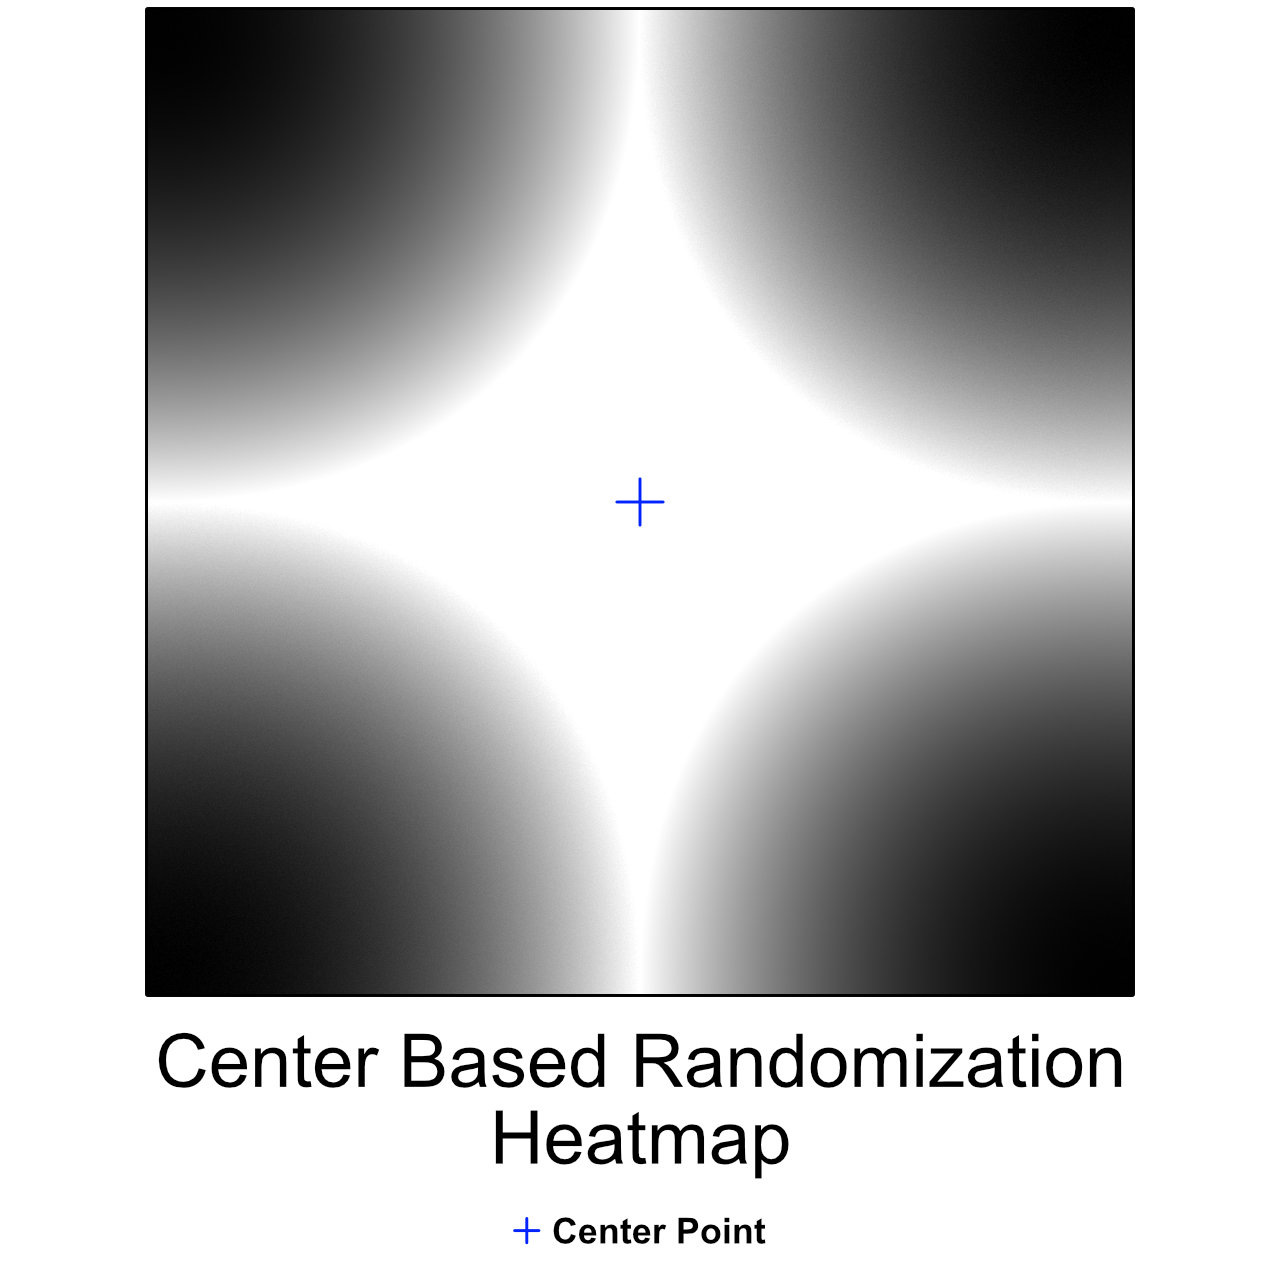
\includegraphics[width=0.65\textwidth]{img/cbr-map}
\caption{Heat map of a 2D area of points that are more likely to less likely to be generated from light to dark based on a center point}
\end{center}
\end{figure}

\par The points that are near to the axis of the center point are more likely to be generated than those that are far from the center point when the `deg' is greater than 1. When `deg' is less than 1, points far from the center point are generated more while when `deg' is 1, it is generating a uniform random number only.
